%%
%% titlepage.tex

%%
%% set title page background (has MUN engineering logo in top left corner)
\setbeamertemplate{background}{%
  \begin{tikzpicture}
    %%
    %% define necessary positions and lengths
    \pgfmathsetmacro{\leftlinebnd}{1} % x-coordinate of leftmost point on line
    \pgfmathsetmacro{\lineheight}{1}  % y-coordinate of line
    \pgfmathsetmacro{\logowidth}{1.5}
    \pgfmathsetmacro{\munlogox}{12.8-\logowidth}
    \pgfmathsetmacro{\munlogoy}{1}
    \pgfmathsetmacro{\rightlinebnd}{\munlogox-1}
    \pgfmathsetmacro{\munenglogox}{1.25}
    \pgfmathsetmacro{\munenglogoy}{8.3}
    \pgfmathsetmacro{\themiddlex}{6.4}
    \pgfmathsetmacro{\headerposy}{8.2}
    %%
    %% generate full-slide bounding box for tikz-generated background
    %%   -> sets up coordinate system with length measured in units of cm
    %%   -> origin in bottom left corner, x- and y-axes are def as usual
    %%   -> things to note:
    %%          1) \the\paperwidth returns the string "364.19536pt", which
    %%             is the full width of the slide
    %%          2) \the\paperheight returns the string "273.14662pt" 
    %%             (full height of slide)
    %%    -> define coordinates for the bottom left and top right corners
    \coordinate (bottomleft) at (0,0);
    \coordinate (topright) at (\the\paperwidth,\the\paperheight);
    %%    -> now define the bounding box to be the rectangle defined by
    %%       the bottomleft and topright corners
    \useasboundingbox (bottomleft) rectangle (topright);
    %%
    %% define other important coordinates in terms of positions/lengths 
    %% defined above
    \coordinate (leftLinePt) at (\leftlinebnd,\lineheight);
    \coordinate (rightLinePt) at (\rightlinebnd,\lineheight);
    \coordinate (munLogo) at (\munlogox,\munlogoy);
    \coordinate (munEngLogo) at (\munenglogox,\munenglogoy);
    \coordinate (header) at (\themiddlex,\headerposy);
    %%
    %% draw bounding line
    \draw[munRed,thick] (leftLinePt) -- (rightLinePt);
    %%
    %% draw "Marine Icing Research" header
    \node at (header) {\Large{\textbf{Marine Icing Research}}};
    %%
    %% draw MUN logo in bottom right corner
    \node at (munLogo) {
\includegraphics[width=1.5cm]{img/MUN_Logo_RGB.png}};
    %%
    %% draw MUN engineering logo in top left corner
    \node at (munEngLogo) {
\includegraphics[width=1.5cm]{img/MUN_Eng_Logo.jpg}};
    %%
    %% add picture
    \node at (\themiddlex,3.25) {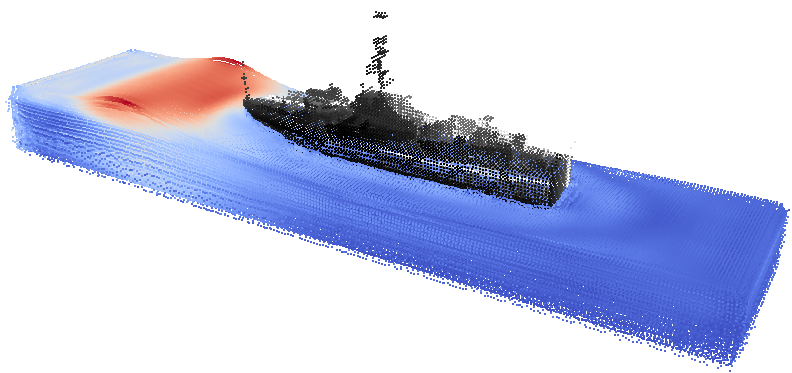
\includegraphics[height=4cm]{img/shipwave.png}};
    %%
    %% add date, place
    \node at (2,0.8) {\tiny{St.~John's, NL, 2016}};
  \end{tikzpicture}
}

%%
%% the title page
\begin{frame}
  \titlepage
\end{frame}
%% M. Sullivan. June, 2016